\documentclass{article}
\usepackage{setspace,tikz}
\usepackage[text={6.5in,8.5in},centering]{geometry}
\geometry{verbose,a4paper,tmargin=2.4cm,bmargin=2.4cm,lmargin=2.4cm,rmargin=2.4cm}
\usepackage{graphicx,amsmath,cases,multirow,appendix,graphicx,xcolor}

\setlength\parindent{0pt}

\newcommand{\note}[1]{\colorbox{gray!20}{#1}}
\newcommand{\ind}{\-\hspace{1cm}}
\newcommand*\circled[1]{\tikz[baseline=(char.base)]{
            \node[shape=circle,draw,inner sep=2pt] (char) {#1};}}

\begin{document}


\noindent\makebox[\textwidth][c]{\Large\bfseries Lecture 4 - Summary}

\rule[0.5ex]{\linewidth}{1pt}
In this class we tried to understand why we (1) need to consider the geometric rather than arithmetic mean lambda when considering population growth, and yet why (2) the arithmetic mean lambda is the appropriate mean to use when determining the expected population size at time $T$.  That may have seemed counterintuitive, so let's clarify and summarize:

When we started contrasting the geometric vs. arithmetic mean, we were talking about the
mean population size of a single population. The average was taken over the $t$ time-points of that population's time-series. The conclusion was that a population growing with (environmental) stochasticity will exhibit a lower average population size over the course of time than will an otherwise equivalent population experiencing less/no stochasticity. For a single focal population, it is it's geometric mean that must be evaluated to determine whether it will grow indefinitely. Alternatively
stated with Case's approximation, $\ln (\bar{\lambda}) > \sigma_{\lambda}^2 / 2 \bar{\lambda}^2$ is needed for the population to grow indefinitely.

\begin{center}
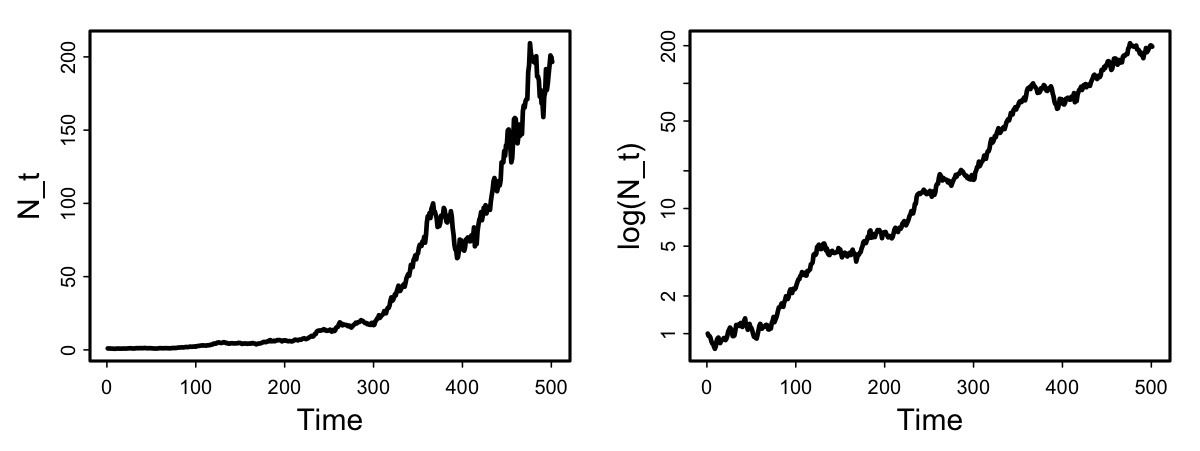
\includegraphics[width=8cm]{figs/image0}
\end{center}

When we proved that $E[N_T]=N_0 \bar{\lambda}^T$ (corresponding to the intuition from our deterministic model), were were asking a different question. That is, we were asking what the expected (mean) population size would be at time T if we were to have followed a whole set of ``replicate'' populations (e.g., if we'd repeated an experiment $n$-times). In other words, the question was: what would the average population size be at time T, averaged across all replicate populations? In this case the arithmetic mean lambda is appropriate.

\begin{center}
 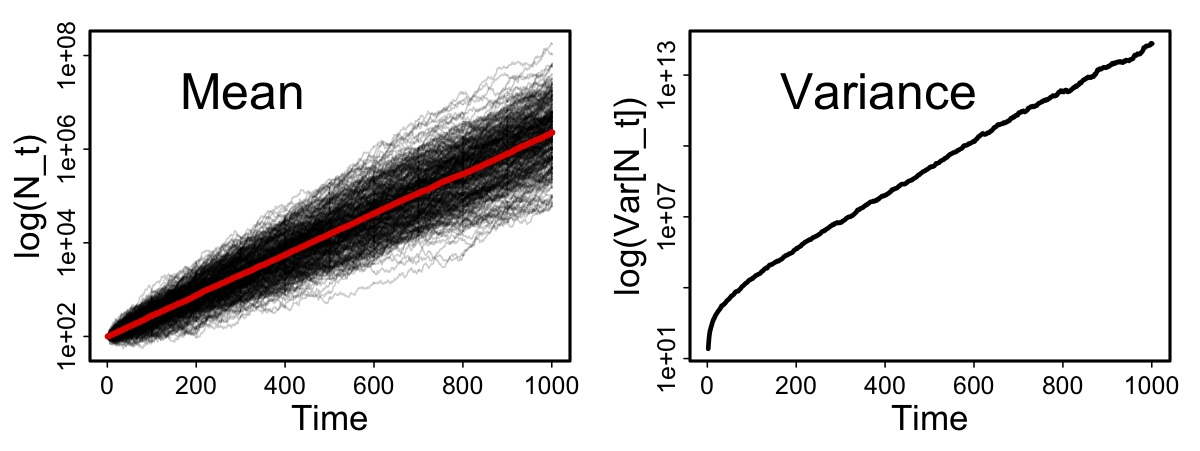
\includegraphics[width=8cm]{figs/image2}
\end{center}

To maybe give you a little intuition for why this is (not just by way of ``proof'', take a look at the following figure. Notice especially on the left hand side (natural scale y-axis) that most populations have a relatively low population size at the final time, but some rare populations have a huge population size. Those huge population sizes counterbalance the rare population sizes. Plotted on a log-scale, you see that distribution of final population sizes looks (and is) more normally distributed.
The average slope of those lines = the arithmetic mean lambda.

\begin{center}
 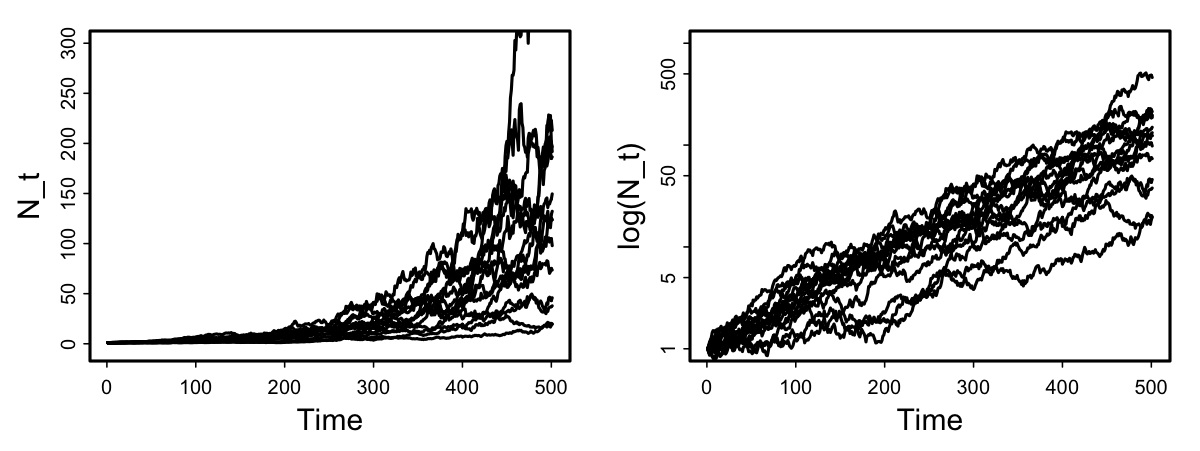
\includegraphics[width=8cm]{figs/image1}
\end{center}

Hope that helps!

\rule[0.5ex]{\linewidth}{1pt}
\end{document}